\documentclass{article}

% if you need to pass options to natbib, use, e.g.:
%     \PassOptionsToPackage{numbers, compress}{natbib}
% before loading neurips_2018

% ready for submission
% \usepackage{neurips_2018}

% to compile a preprint version, e.g., for submission to arXiv, add add the
% [preprint] option:
%     \usepackage[preprint]{neurips_2018}

% to compile a camera-ready version, add the [final] option, e.g.:
\usepackage[final]{nips_2018}

% to avoid loading the natbib package, add option nonatbib:
%     \usepackage[nonatbib]{neurips_2018}

\usepackage[utf8]{inputenc} % allow utf-8 input
\usepackage[T1]{fontenc}    % use 8-bit T1 fonts
\usepackage{hyperref}       % hyperlinks
\usepackage{url}            % simple URL typesetting
\usepackage{booktabs}       % professional-quality tables
\usepackage{amsfonts}       % blackboard math symbols
\usepackage{nicefrac}       % compact symbols for 1/2, etc.
\usepackage{microtype}      % microtypography
\usepackage{graphicx} 
\usepackage{float}
\usepackage{subcaption}

\title{Transfer Learning for Dog Breed Identification}

% The \author macro works with any number of authors. There are two commands
% used to separate the names and addresses of multiple authors: \And and \AND.
%
% Using \And between authors leaves it to LaTeX to determine where to break the
% lines. Using \AND forces a line break at that point. So, if LaTeX puts 3 of 4
% authors names on the first line, and the last on the second line, try using
% \AND instead of \And before the third author name.

\author{%
  Yizhou Chen\\
  \texttt{yic244@ucsd.edu} \\
  \And
  Zhongke Ma\\
  \texttt{z2ma@ucsd.edu} \\
  \And
  Qichao Zheng\\
  \texttt{q5zheng@ucsd.edu} \\
  \And
  Yisheng Ji\\
  \texttt{y3ji244@ucsd.edu} \\
}

\begin{document}
% \nipsfinalcopy is no longer used

\maketitle

\begin{abstract}
  In this project, we achieve classification of dog breeds from Stanford Dog Dataset which contains images of 120 dog breeds. ResNet50, DenseNet, VGG19 and InceptionV3 were used to extract the features. To get a better accuracy, we apply transfer learning on different networks such as VGG19 and InceptionV3. These networks were already built on Keras, which is a deep learning library and provides some popular neural networks. The result of this project can be used in identification of dogs in images.
\end{abstract}

\section{Introduction}

\subsection{Motivation}

Dog have become more and more important in our daily life, they appear as pets, transportation, drug detector and so on. Since different breed of dogs can help people in different way, the identification on breed of dogs have become commonly mentioned nowadays in many fields. Thus, we need a more accurate and efficiency way to classify the breed of dogs.


\subsection{Convolutional Neural Network}

Deep learning models have achieved remarkable results in computer vision in recent years. [1] As one of the deep learning networks, Convolutional Neural Network has widely used around the world for image classification. The CNN consist of neurons and the weights and biases of the neurons can be trained. Each neuron receives some inputs, performs a dot product and optionally follows it with a non-linearity. Convolutional layer, pooling layer, and fully-connected layer are the three main types of layers of Convolutional Neural Network.

In order to improve the performance of the network, CNN model nowadays has become deeper. However, as CNN become deeper, the cost of time and computing resource also become larger. Thus, to save time and make our calculation more efficient, we will use a pre-trained model in our project. Pre-trained model is a model already trained for some other task, we can re-train them in order to fit our task.

\begin{figure}[H]
	\centering
	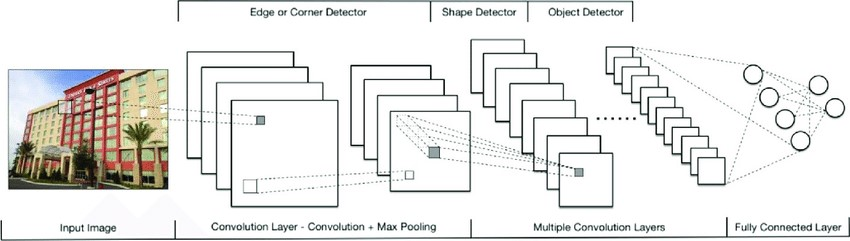
\includegraphics[width=3.5in]{pics/CNN} 
	\caption{Basic structure of CNN.}
\end{figure}

\section{Description of methods}

In this project, we will adopt several CNN models for the purpose of image classification. 
The past ten years have witnessed great success in the performance of deep network handling the problem of image classification. 
And there have been serverl great framewark or architectures successful achieve below the $5\%$ top five error rate. 
Such as the \textbf{DenseNet}, \textbf{ResNet} and \textbf{Inception}. 
The former two methods adopt the concepts of \emph{shortcut connections}, while the latter one utilize the manner of \emph{factorizing convolutions}. 
The purpose of these methods is inituitive, by reducing the parameter of deep network so as to allow for the network to grow deeper and deeper. 

Therefore, in this project, we wish to explore the difference between these methods. 
Namely, we wish to see the difference of \emph{a) shortcut connections} and \emph{b) factorizing convolutions} in perforing large scale, multi-labeled image classifications.
Unlike the basic classifcation problems, where the objects being classified varied in a wide range.  
In this projects, we wish to examine how well the deep network can handle the classification of similar objects. Given thst thoes target objects of the same catagory can somehow varied in a wode range. 

Further, we compare the performance of \textbf{DenseNet} and \textbf{Inception V3}, together with a earlier framework \textbf{VGG19}, to examine the performance under different deep network.

\subsection{VGG19}
VGG is a network of increasing depth using an architecture with very small convolution filters. With small convolution filters, the number of parameters can be reduced. The input of VGG is 224*224 RGB images. Then the input image will go through the convolutional layers, where filters with a small receptive field will be applied. Each convolutional layer has different depth, some of the convolutional layers will have a max-pooling layer followed, and the max-pooling layer has a 2$\times$2 pixels window with stride 2. With max-pooling layers, VGG can achieve spatial pooling. After the stack of convolutional layers three fully connected layers are followed. The first two layers have 4096 channels each, the third have 1000 channels. And the last layer of the network is a soft max layer. After the input go through the whole network, the output will be classification contains 1000 channels. VGG16 and VGG19 are the two most common models of VGG. VGG 16 has 16 weight layers which has about 138 million of parameters in total, while VGG19 has 19 weight layers which has about 144 million of parameters in total. [4] The model we will use in our project is VGG19, it can achieve 7.3\% top 5 error in ILSVRC.

\begin{figure}[H]
	\centering
	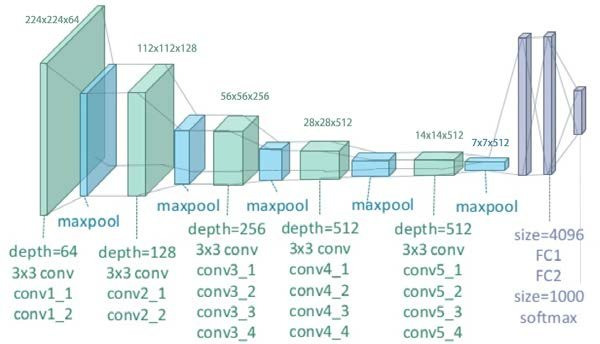
\includegraphics[width=0.8\linewidth]{pics/vgg} 
	\caption{VGG19 architecture.}
\end{figure}

\subsection{DenseNet}

More and more models have shown that convolutional neural networks can become substantially deeper, more accurate, and efficient to train if they contain shorter connections between layers close to the input and those close to the output. Thus, Dense Convolutional Networks (DenseNet) was introduced. DenseNet consists of dense block, within each dense block, each layer is connected to every other layer in a feed-forward fashion. [3] In DenseNet, every layer is connected together by dense connectivity in order to have max information flow between the layers which means every layer have multiple inputs from other layers. 

In DenseNet, fewer parameters is needed, which means the parameters in DenseNet can be more efficiency than traditional neural networks. Besides, DenseNet can be deep while the layers can be slim. With all these advantages, DenseNet is easily to be trained.

\begin{figure}[H]
	\centering
	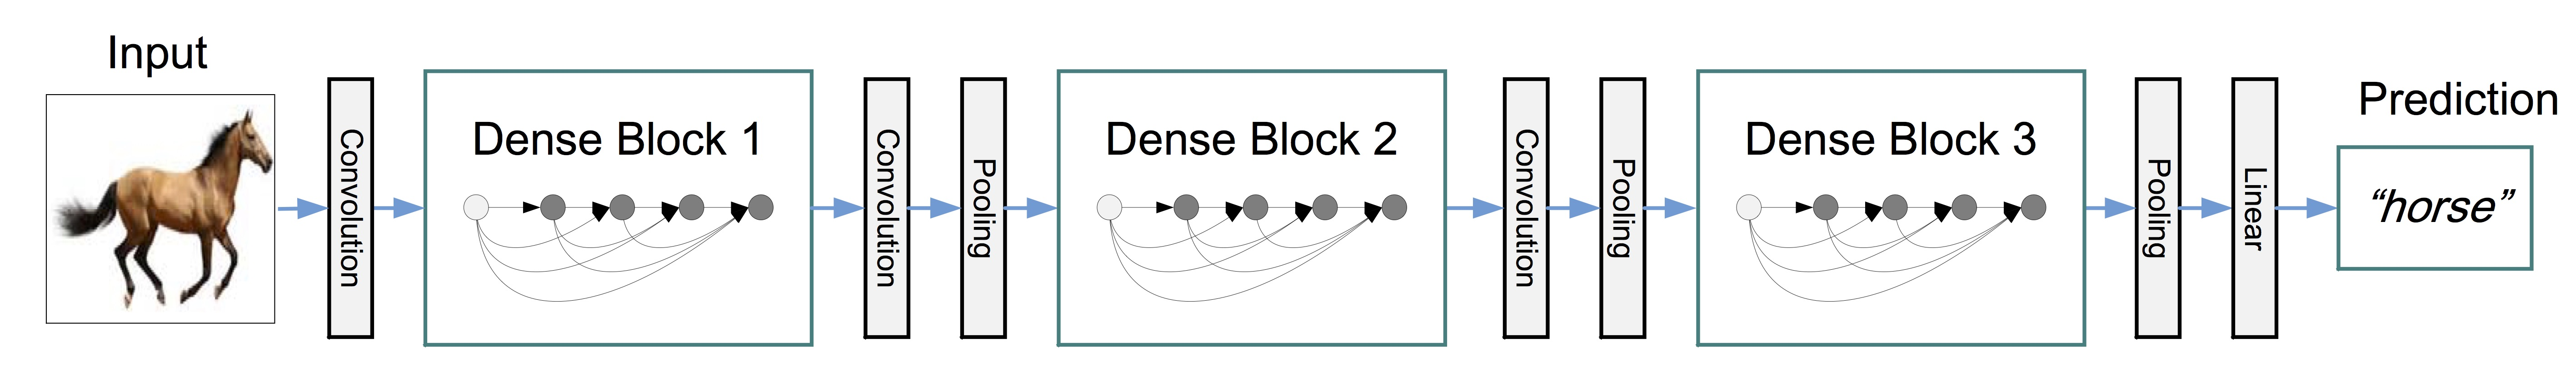
\includegraphics[width=0.8\linewidth]{pics/densenet} 
	\caption{A deep DenseNet with three dense blocks.}
\end{figure}

\subsection{InceptionV3}

Inception is a deep convolutional neural network which provides a new state of the art for classification and detection. It makes a better use of the computing resources inside the network and makes the network deeper and wider while the computing budget is not affected. Inception networks consist of Inception modules. The main idea of the Inception architecture is to consider how an optimal local sparse structure of a convolutional vision network can be approximated and covered by readily available dense components. [5] To find the optimal local sparse structure, we assume that each unit of the previous layer refers to some part of the input image, which can find the clusters that focused on some particular region, thus, these clusters can be summed up by a 1*1 convolution in the following layer. And to avoid patch-alignment problem, the filter size of Inception has only 3 options: 1$\times$1, 3$\times$3 and 5$\times$5. To keep the computing complexity stable, Inception network uses dimensionality reduction which can reduce the feature maps from 192 to 16.

InceptionV3, as the improved model of Inception networks, has 42 layers, which is much deeper than GoogLeNet, the first model of Inception networks. The improvement InceptionV3 make is that they applied factorization of convolutions and improved normalization in the networks. [6] Comparing with GoogLeNet, the top 5 error of InceptionV3 is improved from 6.67\% to 4.49\%.

\begin{figure}[H]
	\centering
	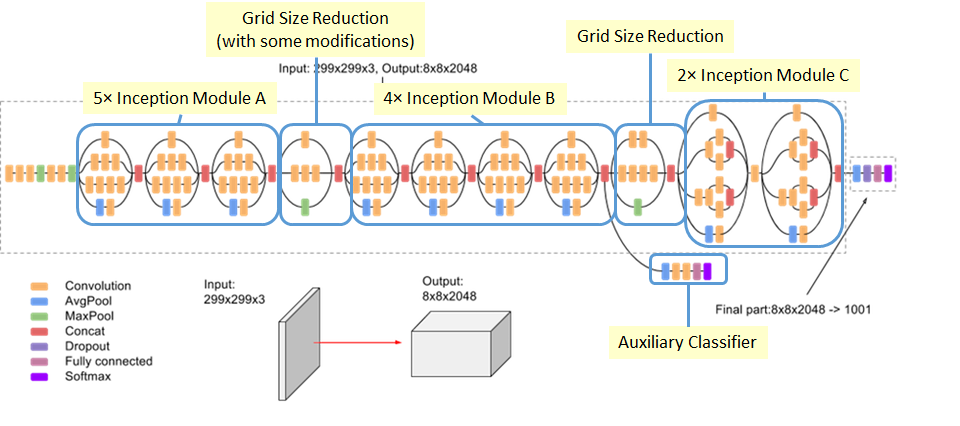
\includegraphics[width=0.8\linewidth]{pics/inception} 
	\caption{InceptionV3 architecture.}
\end{figure}

\subsection{Transfer learning}

Transfer learning is a machine learning technique where a model trained on one task is re-purposed on a second related task. 
In traditional CNN for image classification, usually the earlier layers are to detect edges, while deeper layers will try to detect some specific features. 
With transfer learning, we can use the earlier layers to re-train the deeper layers. The main benefit transfer learning is saving training time without hurting the performance. Also, with transfer learning, we can use less data to train the neural networks. 

\section{Implementation Details}

In this section, we will brefily introcude how we implemented and modified these three deep network mentioned above. 
\subsection{Models}
Basically, we first examine the performance of these three pretrained network on our testing set; then we remove the final layers (top layers) within the pretained models, plugged a new fully-connected layers as the new classifer. 
During training, we first forzen the parameters of previous layers, since they all have been properly trained and fine-tuned, and trend to achieve optimal performance on general classification problems. 
These previous layers, then functioned as feature extarctor, extracting the features from the input image tensors, generating a group of feature vectors, passing through the last fully connected layer, and fire on some specfied output nodes indicating the predicted catagories of the input images. 

Table~\ref{tab:1} demenstartes one of the prototype of the deep network that will be adopted in our project. 

\begin{table}[h]
	\centering
	\caption{A typical modified framework for our project.}
	\label{tab:1}
	\begin{tabular}{ccc|ccccccc}
		\toprule
		& layer &&& function && input dims && output dims & \\ 
		\midrule
		& $0$ &&& \emph{input images} && $(n, 3, 224, 224)$ && -- & \\ 
		& $\cdots$ &&& -- && -- && -- & \\
		& $n-1$ &&& \emph{extract deep features} && -- && $(n, n, n, 2048)$  & \\ 
		\midrule
		& $n$ &&& \emph{global average pooling} && $(n,n,n, 2048)$ && $(n, 2048)$ & \\ 
		& $n+1$ &&& \emph{drop out} && $(n, 2048)$ && $(n, 2048)$ & \\ 
		& $n+2$ &&& \emph{fully connected} && $(n, 2048)$  && $(n, 120)$ & \\ 
		\bottomrule
	\end{tabular}
\end{table}
\subsection{Dataset}
As for the dataset, we have $12,000$ samples for training and $8,580$ samples for testing. We further adopted the method of data augmentation to enhance the numbers of the training set. More specifily, we adopt some random \emph{shifts}, \emph{zooms}, \emph{rotates} and \emph{filps} to tarnsform the origin image, so as to obtained the augmented data for training. This method, does somehow improve the performance of our model. 
\subsection{Losses}
As for the loss function, we basically use both the \emph{categorical\_crossentropy} and \emph{sparse\_categorical\_crossentropy} that are typically adopted in classification problem. 
Also, by some literature review, we have also try to adopted the \emph{center loss} $\mathcal{L}_C$, as a regualrized term for the training of our model, which is found to be significant useful in classifying similar targets. Therefore, we define the loss of our model as
\begin{equation}
\mathcal{L}  =  \mathcal{L}_S + \lambda \mathcal{L}_C 
\end{equation} 
where $\mathcal{L}_S$ is the softmax loss and $\mathcal{L}_C$ is the center loss defined by
\begin{equation}
	\mathcal{L}_S = - \sum_{i=1}^{m} \log  \frac{e^{W^T x_i + b_{i}}}{\sum_{j=1}^{n} e^{W^T x_j + b_{j} }} 
\end{equation}
\begin{equation}
	\mathcal{L}_C = \frac{1}{2} \sum_{i=1}^{m} \left\Vert x_i - c_i\right\Vert^2_2
\end{equation}

\section{Experimental Settings}
\label{sec:ex}

\subsection{Datasets}
The dataset we used in this project is Stanford Dogs Breed Dataset, which contains images of $120$ breeds of dogs from around the world, such as Chihuahua, Japanese spaniel and Rhodesian ridgeback. This dataset has been built using images and annotation from ImageNet for the task of fine-grained image categorization. There are totally $20,580$ images in this dataset, with $12,000$ images in the training set and $8,580$ in the testing set.

For training-validation split rate, wo use $1/6$ and introduce data augmentation methods including left/right shifting $\pm 0.2$, scaling $1 \pm 0.2$, rotation $\pm 30$ and horizontal flip. 
The training, testing and validation data in a batch scale of $32$ samples per batch, and in total we have $315$ batches for training, $60$ batches for validation and $269$ batches for testing. Figure~\ref{fig:5} shows $10$ sample images from the dataset with class label of \emph{Border Collie}. 

\begin{figure}[H]
	\centering
	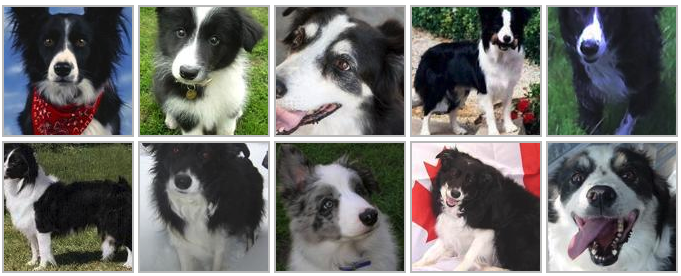
\includegraphics[width=0.7\linewidth]{pics/dogs} 
	\caption{Sample Images from the Stanford Dogs Breed Dataset. Catagory =\emph{Border Collie} }
	\label{fig:5}
\end{figure}

\subsection{Training Parameters}
Undoubtly, the most important and most difficult part of trainning a deep network, is how to properly choose the \emph{1)} layers, \emph{2)} losses and \emph{3)} optimizers. All these staffs are characterized by parameters and closely related with the performance of the whole network. 
Table~\ref{tab:2} demenstartes some of the parameters that we adopted for training the plugged layers. 

\begin{table}[h]
	\centering
	\caption{A typical modified framework for our project.}
	\label{tab:2}
	\begin{tabular}{c|ccccc}
		\toprule
		 plugged layer & activations & optimizeor & step / epoch & loss & early stopping\\ 
		\midrule
		 fc64, fc120 & ReLu, Softmax & adam + sgd & 120 & $\mathcal{L}_S$ & \emph{true} \\ 
		 d0.2, fc120 & --, Softmax & sgd & 80 & $\mathcal{L}_S$ & \emph{true} \\ 
		 d0.4, fc120$\times$2 & --, Softmax & adam + sgd & 120 & $\mathcal{L}_S$ & \emph{true} \\
		 fc64, fc120 & GLU, Softmax & adam + sgd & 120  & $\mathcal{L}_S + \mathcal{L}_C$ & \emph{true} \\ 
		\bottomrule
	\end{tabular}
\end{table}

As for finetuning, we adopt a two-step finetune manner. 
Namely, we fine-tune the network for two stages, while in the first stage, we use the less augmented data, with only left/right shifting $\pm 0.1$ and scaling $1\pm0.05$. 
And for the second stage, we use the non-augmented data, simply set all augment manner to \emph{false}. 
As for the optimizer, we again, utilize sgd, with a learning rate of $0.0001$ and momentum of $0.9$. 
For each stage, we run for $200$ epochs with a step size of $120$ batches per epoch, toger ther with early stopping if the validation loss start to increase. 

\subsection{Hardware \& Framework}
For the whole project, we use the \emph{Keras} along with the \emph{Tensorflow} backend, running on both the UCSD's MLDSP Clusters equipped Ndivda GeForce 1080Ti and our both PC with GeForce 1060. 
To avoid the problem of packages' version compatibility, we adopted the offical \emph{tensorflow}'s docker. 

\section{Results}

\subsection{VGG19}
As the forerunner of deep network in image classification, \emph{VGG19} does somehow introduce some very important concepts, such as \emph{going deeper}, \emph{reduce parameters}. 
It is very basic model in understanding how \emph{convolutional neural network} can be experted in classifying images. 
Therefore, we first examine the performance of \emph{VGG19} under our experimental settings as described in Section~\ref{sec:ex}.

The orginal \emph{VGG19} network have $19$ weighted layers and with the last flatten layers given a output of $(1, 25088)$ feature vector. 
Followed by $3$ fully connected layers with $4096$, $4096$ and $1000$ outputs each. 
This however, for our dataset with onlt $120$ classes, seems a litte trival. 
Table~\ref{tab:vgg19} described the details of our modified \emph{VGG19} network. 
\begin{table}[h]
	\centering
	\caption{\emph{VGG19} Plugged Layers}
	\label{tab:vgg19}
	\begin{tabular}{c|ccc}
		\toprule
		layer & input dims & output dims & comments \\
		\midrule
		\emph{fc} & $(n, 25088)$ & $(n,4096)$ & \emph{fixed} \\
		\emph{dropout} & -- & -- &  $r =  0.5$ \\
		\emph{fc} & $(n,4096)$ & $(n,120)$ & \emph{predictions} \\
		\bottomrule
	\end{tabular}
\end{table}

\begin{figure}[htb]
	\centering
	\label{fig:res}
	\begin{subfigure}{0.48\linewidth}
		\centering
		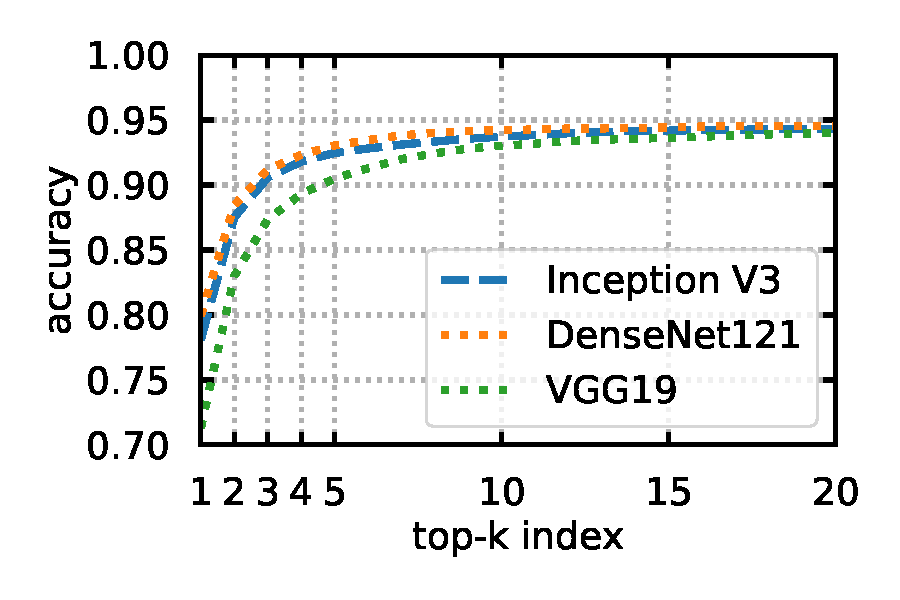
\includegraphics[width=\linewidth]{pics/Model_naive}
		\caption{Results of $3$ Naive Models}
		\label{fig:all3}
	\end{subfigure} 
	\begin{subfigure}{0.48\linewidth}
		\centering
		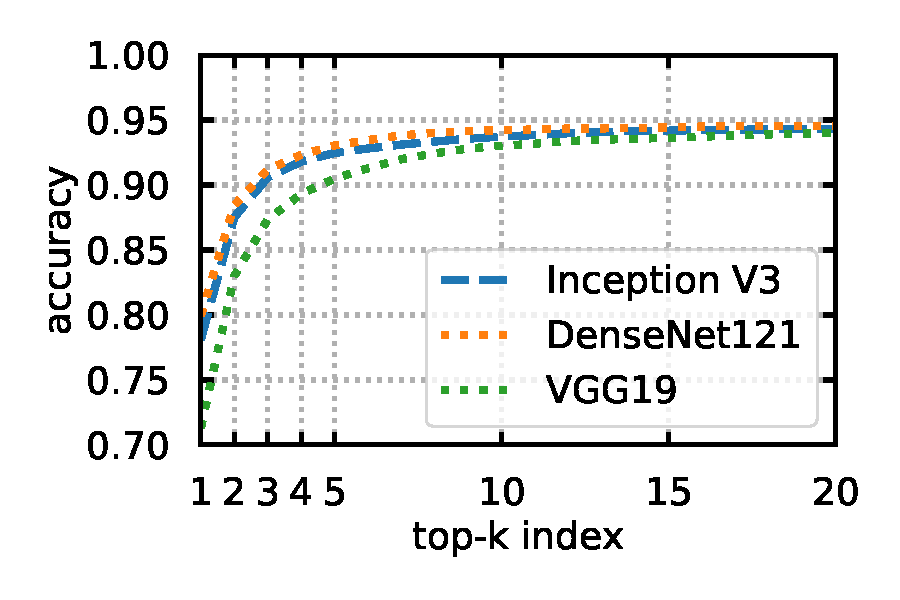
\includegraphics[width=\linewidth]{pics/Model_naive}
		\caption{Results of \emph{VGG19}}
		\label{fig:vgg19}
	\end{subfigure} 
	\begin{subfigure}{0.48\linewidth}
		\centering
		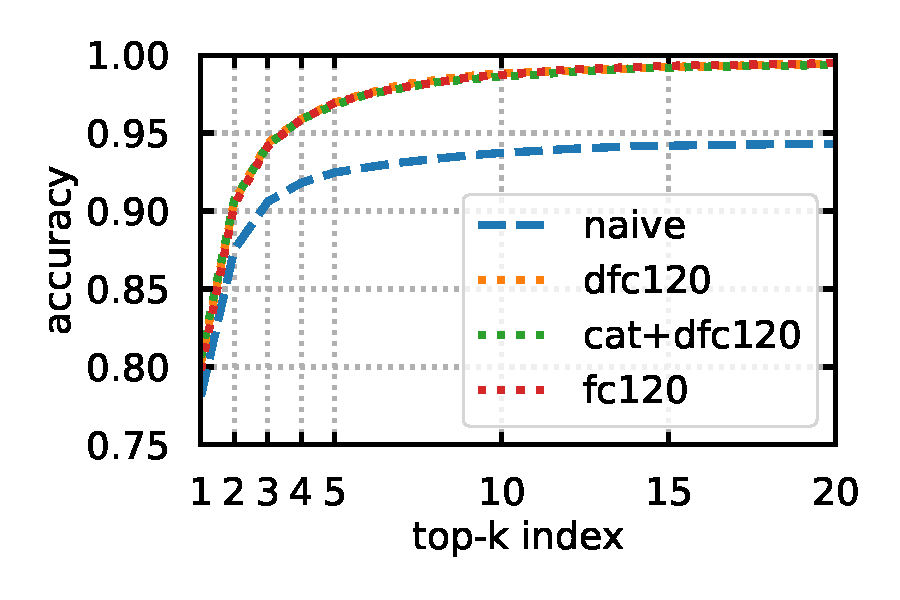
\includegraphics[width=\linewidth]{pics/InceptionV3}
		\caption{Results of \emph{Inception V3}}
		\label{fig:incetionp}
	\end{subfigure} 
	\begin{subfigure}{0.48\linewidth}
		\centering
		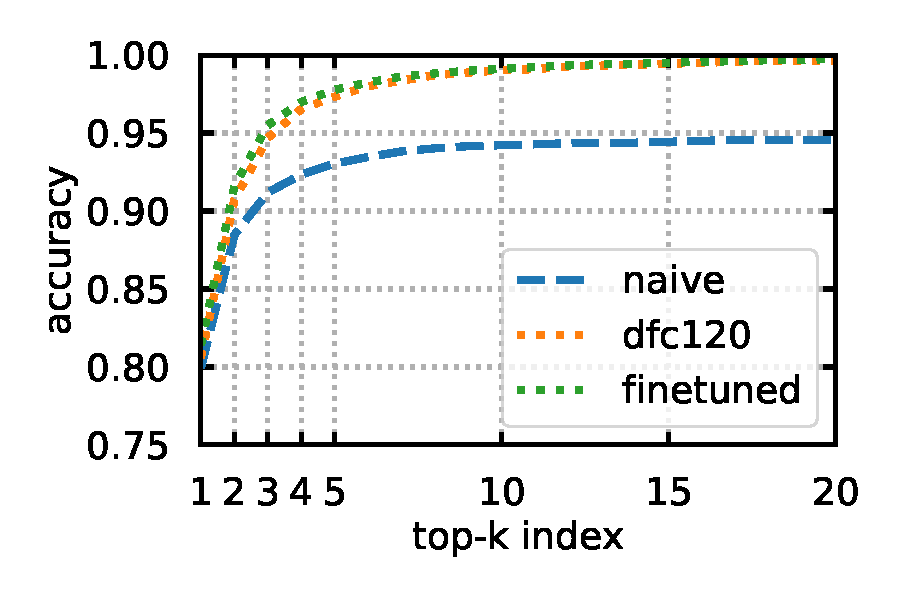
\includegraphics[width=\linewidth]{pics/DenseNet}
		\caption{Results of \emph{DenseNet}}
		\label{fig:densenet}
	\end{subfigure} 
	
	\caption{Results of Top-$k$ Accuracy Verses $k$ index}
\end{figure}


\subsection{InceptionV3}
We further explored the effects different plugged layers based on \emph{Google}'s \emph{Inception V3} model. 
Results of those methods are ploted in the form of \emph{top-k accuracy verse k index}, as in Figure~\ref{fig:incetionp}

Noted that, by implementing \emph{fully-connected} layers with / without \emph{dropout} layers can results in significant difference, 
this is because the neural networks are, by natura, likely to be overfitted, especially in case of multi-layer classifier. 
Also, 

\subsection{DenseNet121}
Counting on the results from \emph{InceptionV3}, we modified and trained the \emph{DenseNet121} network with only plugged \emph{dfc120} layers. Cause it can amlost achieve the same performance among the other architecture without introducing more parameters. 
The final \emph{Dense Block} outputs a tensor with only $1024$ dimensions, 

Figure~\ref{fig:densenet} shows the performance of our modified \emph{DenseNet} model. 

\subsection{Comparision}

\subsection{Success Cases}
\subsection{Failures}

\newpage
\section{Discussion}

\subsection{Inference}
\subsection{Conclusion}
\subsection{Learning}
\subsection{Challenges}
For the purpose of classifying the breed of dogs properly, several challenges exist to be solved: 
\begin{itemize}
	\item[1] there are many breeds of dogs in the world, which means the computer vision algorithm needs to take into consideration a great number of categories. And based on No-Free-Lunch-Theorem, with the number of dogs' breeds increasing, the accuracy of dog classification will decrease to some extent; 
	\item[2] some breeds of dogs have very similar appearance, such as Samoye and Japanese Spitz, Bichon Frise and Teddy dog, Chihuahua and Minlature Pinscher, etc. Some of these dogs are even too similar for human beings to distinguish from one another. Therefore, how to accurately classify these similar dogs is a big challenge; 
	\item[3] the third lies in the fact that we only have access to limited number of training images per class, which means we need to make the best use of the images to extract the features of different kinds of dogs. Therefore, we need to find a good way to process the original images to get as much information as possible. 
\end{itemize}
\subsection{Feture Work}

\section{Appendix}


\section*{References}

\medskip

\small

[1] Kim Y. Convolutional neural networks for sentence classification[J]. arXiv preprint arXiv:1408.5882, 2014.

[2] He K, Zhang X, Ren S, et al. Deep residual learning for image recognition[C]//Proceedings of the IEEE conference on computer vision and pattern recognition. 2016: 770-778.

[3] Huang G, Liu Z, Van Der Maaten L, et al. Densely connected convolutional networks[C]//CVPR. 2017, 1(2): 3.

[4] Simonyan K, Zisserman A. Very deep convolutional networks for large-scale image recognition[J]. arXiv preprint arXiv:1409.1556, 2014.

[5] Szegedy C, Liu W, Jia Y, et al. Going deeper with convolutions[C]//Proceedings of the IEEE conference on computer vision and pattern recognition. 2015: 1-9.

[6] Szegedy C, Vanhoucke V, Ioffe S, et al. Rethinking the inception architecture for computer vision[C]//Proceedings of the IEEE conference on computer vision and pattern recognition. 2016: 2818-2826.


\end{document}
